\documentclass{article}

\usepackage{amsfonts}
\usepackage[colorlinks=true,citecolor=blue,urlcolor=cyan,linkcolor=red]{hyperref}
\usepackage{amssymb}
\usepackage{amsmath,amssymb,amscd,epsfig,amsfonts,rotating, bm}
\usepackage{graphicx}
\usepackage{epsfig}
\usepackage{multirow}
\usepackage{booktabs}
\usepackage{url}
\usepackage[margin=1.5in]{geometry}

\newtheorem{def:def}{Definition}
\newtheorem{thm:thm}{Theorem}
\newtheorem{thm:lm}{Lemma}

\DeclareMathOperator*{\argmax}{arg \, max}
\DeclareMathOperator*{\var}{var}
\DeclareMathOperator*{\cov}{cov}
\newcommand{\bs}{\boldsymbol}

\title{A Practical Comparison of Denoising Autoencoder and Factorization Machine for Recommending Movies\\
	\Large{CS420 Coursework: Recommender System}}
\author{Runzhe Yang\\
{\small RzAlpaca, 5140309562} \\
{\small Shanghai Jiao Tong University}\\
{\small \textsf{yang\_runzhe@sjtu.edu.cn}}}
\begin{document}
\maketitle

\begin{abstract}
In this coursework, the author implemented and compared two most successful models for Recommender System: Denoising Autoencoder (DAE) and Factorization Machine (FM). Although the DAE is a powerful unsupervised deep learning method to recover corrupted data, on the specific recommender system task it is still less powerful than traditional method such as the FM, because of the high sparsity of data and poor compatibility with side information.
\end{abstract}

\section{Introduction}\label{sec:intro}
\subsection{Background}\label{sec:bg}
The objective of a Recommender System is to automatically recommend some items or goods satisfying users, based on users behavioral history. The input data of a Recommender System is varied. Generally speaking, it can be divided into four main parts: 
\begin{itemize}
	\item User: user IDs, age, gender, number of watched movies, etc..
	\item Item: item IDs, category, release data, number of watchers, etc..
	\item Time: year, month, week, hour, etc..
	\item Observed ratings.
\end{itemize}
The output of a Recommender System is the prediction of some user's rating on some item. Inputs other than user IDs and item IDs and given ratings are called side information.  Tuples $\langle userid, itemid, rating\rangle$ composed a sparse user-item rating matrix $R$. The goal of Recommender System can be restated as the blank filling in $R$ with or without the auxiliary side information.

If only the sparse $R$ is given, a traditional model of recovering $R$ is the so-called {\em topic model}, which assume $R$ is low-ranked and is the production of two small matrix $U$ and $V$. Suppose there are $u$ users and $i$ items and $R$ is rank $t$. Then $R = UV^T$ indicates that the size of $R$ is $u\times i$, the size of $U$ is $u \times t$ and the size of $V$ is $i \times t$. The $t$ here can be interpreted as the number of topics. Therefore, $U$ and $V$ are user preference matrix and item attribute matrix in fact .


%\begin{table}
%\small
%\renewcommand{\arraystretch}{1}
%\centering
%\caption{Notations and descriptions}\label{tab:notation}
%\resizebox{0.8\columnwidth}{!}{
%\begin{tabular}{c|l}
%\hline
%Notation & Description \\
%\hline
%$\bs{x}$ & The pre-defined value of positive user response. \\
%$y$ & The true label of user response. \\
%$L(\bs{x})$ & The loss function of the objective.\\
%$p$ & The predicted probability $Pr(\hat{y}=1|\bs{x})$.\\
%\hline
%\end{tabular}
%}
%\end{table}

\subsection{Collaborative Filtering}\label{sec:cf}
The Recommender System based on {\em Collaborative Filtering} use users past behaviors learn implicit information about user preference or similarity among users or items. Basically, there are two general methods: memory-based and model-based methods to do collaborative filtering. The memory-based method includes item-based k-nearest neighbors (knn), user-based knn\cite{} and some variants with time information. These methods regard each item or user as a vector, then a quantitive similarity can be compute. Using pair-wise similarities we can predict a rating based on ratings from similar users or of similar items.

A typical model based method is mentioned in section \ref{sec:bg}, called matrix factorization\cite{}. However, the simple matrix factorization such as SVD has every low capacity to capture the feature of data, and cannot integrate the side information. To address this problem, many variants like SVD++\cite{} and timeSVD++\cite{} are proposed. Deep learning as a advance representation extraction method, such as Autoencoder (AE) is also used in this area to improve the capacity of simple SVD. Factorization Machine can be seen as a generalization of SVD++, which is also a practical model-based method for the Recommender System.

\section{Methodology}\label{sec:method}
In this course work, the author mainly compared two models: Denoising Autoencoder (DAE) and Factorization Machine. 

\subsection{Item-Based Denoising Autoencoder}
\begin{figure*}[!h]
	\centering
	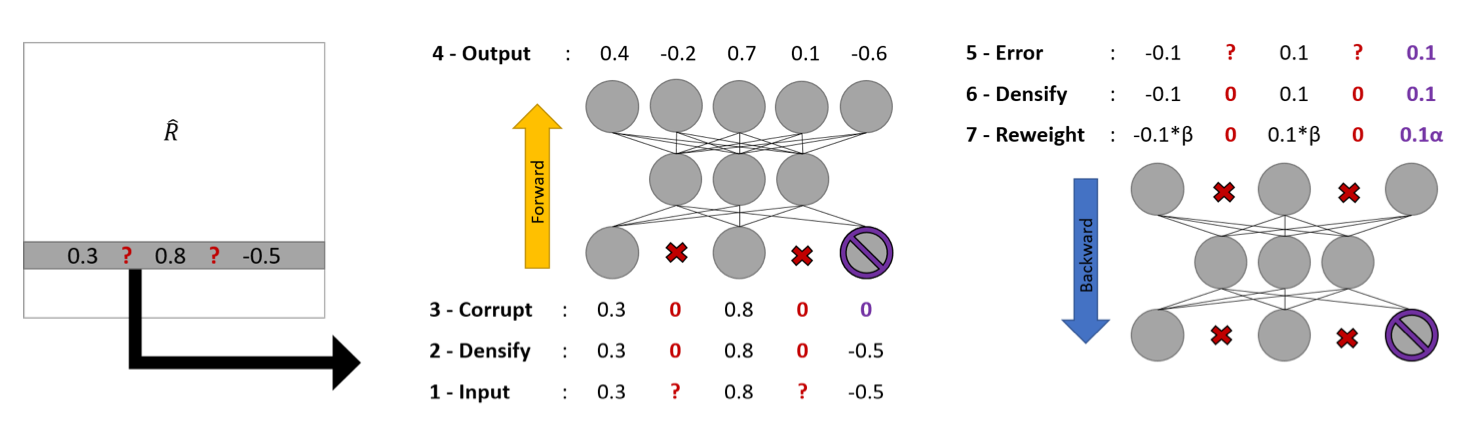
\includegraphics[width=\textwidth]{figures/fig1}
	\caption{This illustration is borrowed from \cite{}. Feed Forward/Backward process for sparse Autoencoders. The sparse input is drawn from the matrix of ratings, unknown values are turned to zero, some ratings are masked (input corruption) and a dense estimate is finally obtained. Before backpropagation, unknown ratings are turned to zero error, prediction errors are reweighed by $\aleph$ and reconstruction errors are reweighed by $\beta$ .}
\end{figure*}

Denoising Autoencoder is a extension of basic idea of autoencoder, which adds some noise to the training data deliberately. The DAE has to learn how to ``reveal the mask". Hence it learns robuster representation for the data, and therefore improves the generalization ability of the model.

For a given sparse rating matrix $R \in \mathbb R_{u\times i}$, a user is represented by a sparse row $u_i\in \mathbb R_i$ and item is represented by a sparse column $v_j \in \mathbb R_u$. The item-base autoencoder use the batch of item vectors $\{v_j\}$ as inputs. If an Autoencoder only has one hidden layer, the corresponding network is $nn(x) = \sigma (W_2 \sigma(W_1 x + b_1) + b_2 )$.
Actually, it is analogue to ``matrix factorization". The predicted vector $\hat v_j$ has the form
\[\hat v_j = nn(v_j) = \sigma\left([W_2'I_u]\left[\begin{matrix}
	\sigma(W_1'v_jb_1)\\
	b_2'
\end{matrix} \right]\right)\]

The training loss is 
\[L_{\alpha, \beta}(\bm x, \tilde{\bm x}) = \alpha\left( \sum_{j\in \mathcal C(\tilde{\bm x}\cap\mathcal K(\bm x)}[nn(\tilde{\bm x})_j - \bm x_j]^2 \right) + \beta \left( \sum_{j\notin \mathcal C(\tilde{\bm x}\cap\mathcal K(\bm x)}[nn(\tilde{\bm x})_j - \bm x_j]^2 \right) + \Omega(\bm W)\]
where $\mathcal K(x)$ are the indices of known values of $x$ and $\mathcal C(x)$ are the indices of corrupted values of $x$.

\subsection{Factorization Machine}

\begin{figure*}[!h]
	\centering
	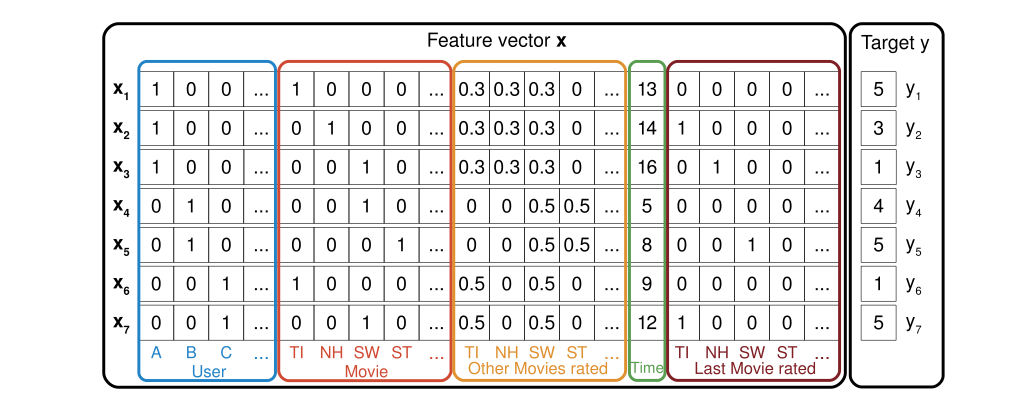
\includegraphics[width=\textwidth]{figures/fig2.png}
	\caption{This illustration is b orrowed from []. Example (from Rendle [2010]) for representing a recommender problem with real valued feature vectors x. Every row represents a feature vector x i with its corresponding target y i . For easier interpreta-tion, the features are grouped into indicators for the active user (blue), active item (red), other movies rated by the same user (orange), the time in months (green), and the last movie rated (brown).}
\end{figure*}
Factorization Machine is proposed to address the feature combination problem of sparse data. For a recommender system, FM can be used as a model exploit all pairwise combination of features. The factorization machine model of order $d=2$ is defined as 
\[\hat y(\bm x) = w_0 + \sum_{j=1}^{p}w_jx_j + \sum_{j=1}^{p}\sum_{j'=j+1}^{p}x_jx_{j'}\sum_{f=1}^{k}v_{j,f}v_{j',f}\]
where k is the dimention of the factorization. While training, we use MCMC to turn the parameters by seeing the model as a probabilistic graph.

\section{Experiments and Results}\label{sec:exps}
\subsection{Data}
There are 94317 users and 99782 items in the given dataset. 5974450 records are the training data. 1524458 records are the test data.

The features the author fed to the model are 
\begin{enumerate}
	\item \texttt{userId}
	\item \texttt{itemId}
	\item \texttt{weekday}
	\item \texttt{hour}
	\item \texttt{movie\_feature1}
	\item \texttt{movie\_feature2}
	\item \texttt{1/number\_of\_watched movies of userId}
	\item \texttt{1/number\_of\_watchers of itemId}
\end{enumerate}

The author also do some observation on the training data. The code is in


 \texttt{``code/RecommenderSystem/data\_observation.ipynb"}
\begin{figure*}[!h]
	\centering
	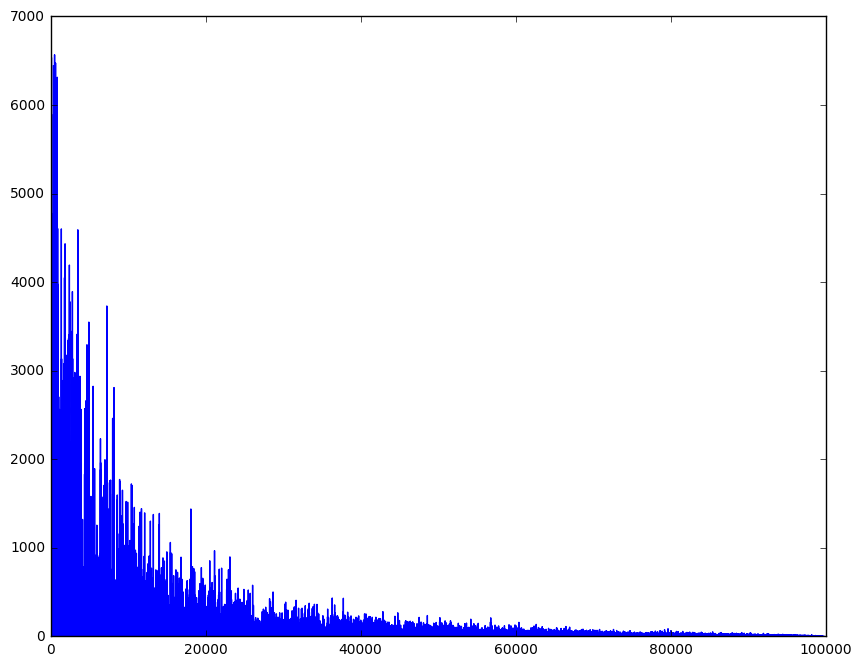
\includegraphics[width=0.6\textwidth]{figures/movie}
	\caption{x-axis: movie id; y-axis: the number of watchers. It is a long-tail distribution.}
\end{figure*}

\subsection{Results}

The best RMSE gained by the Denoising Autoencoder is about 1.51714 on the test set. The best RMSE gained by the Factorization machine is 1.33867. By linearly combining multiple submissions, the author got the final RMSE as 1.32984.


%\begin{figure}[t]
%  \centering
%  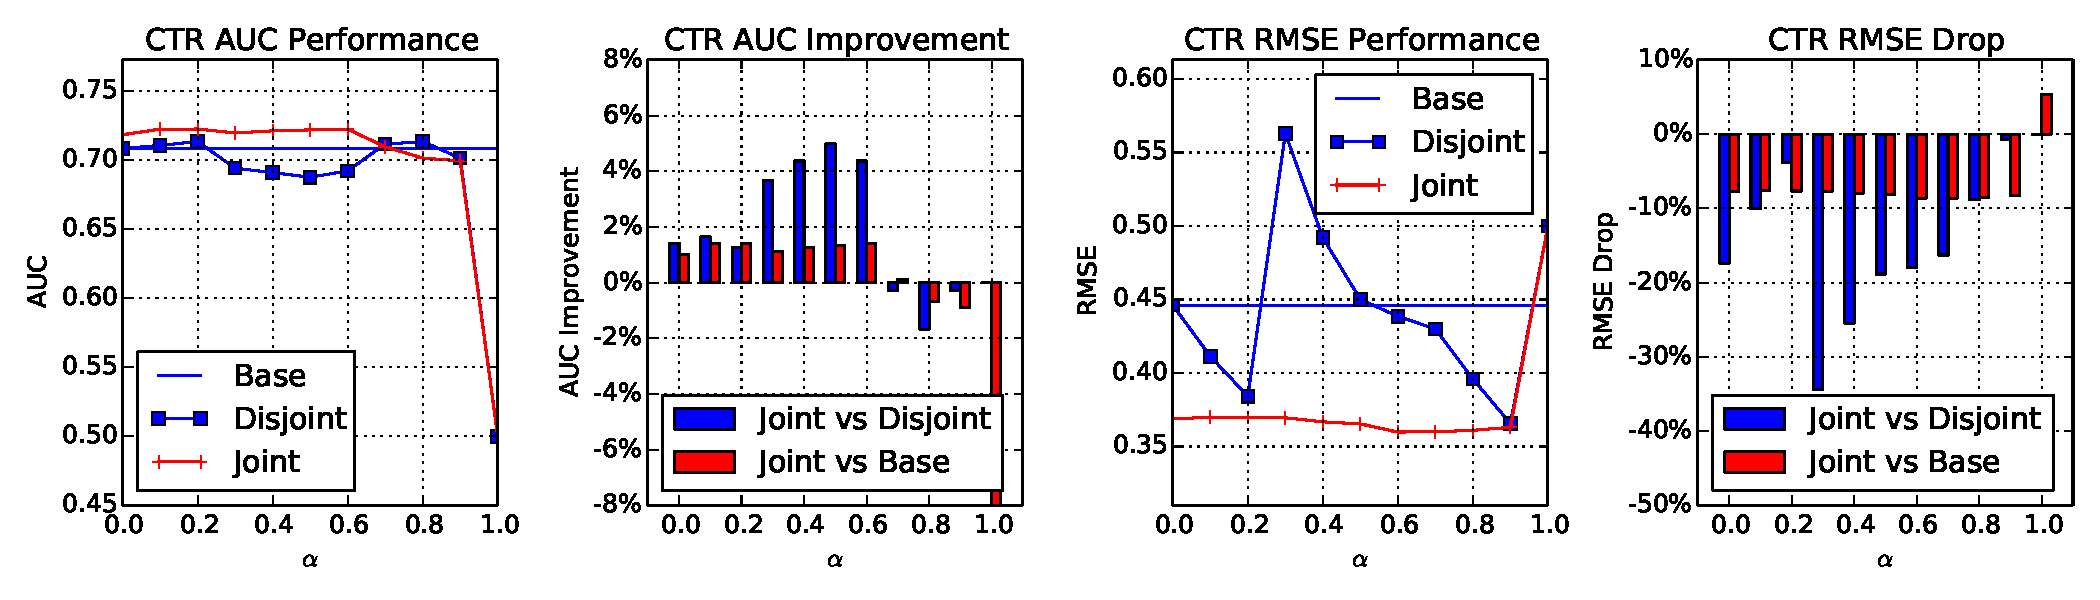
\includegraphics[width=1.0\columnwidth]{figures/basic-perf4.pdf}
%  \caption{The illustration of the performance.}\label{fig:basic}
%\end{figure}

If time permits, I will revise this report \cite{salakhutdinov2007restricted,
wang2015collaborative,
strub2016hybrid,
dong2017hybrid,
rendle2012factorization,
sedhain2015autorec}.

\bibliographystyle{abbrv}
\bibliography{report}


\end{document}
